\clearpage
\phantomsection
\chapter{BACKGROUND AND RELATED WORK}

This chapter surveys the theoretical and technical foundations for the three sub-problems identified in the Introduction, organized in a top-down manner that introduces each topic at the genre level before drilling into its components. Section~1.1 covers Sub-Problem~1 (game engine background): it opens with Roguelike Deckbuilders as a combined genre before separately examining the Roguelike and Deckbuilding mechanics that compose it, then characterizes the balancing challenges unique to the genre. Section~1.2 covers Sub-Problem~2 (AI agent background): motivated by the need for intelligent evaluation agents, it develops the Reinforcement Learning theory including MDP, PPO, invalid action masking, and Domain Randomization. Section~1.3 covers Sub-Problem~3 (optimization background): a survey of game balancing approaches leads into the Genetic Algorithm and NSGA-II, with explicit mapping of each algorithm's parameters to the game-balancing context. Section~1.4 reviews related prior work. Each section closes by connecting the theory to the design decisions in Chapter~2.

\section{Roguelike Deckbuilder Games}

\subsection{Roguelike Deckbuilders}

Roguelike Deckbuilders are a hybrid genre that merges procedural dungeon-crawling with card-driven combat and progressive deck construction. In a typical run, the player traverses a branching map of rooms, fights enemies using a hand drawn from their personal deck, and acquires new cards after victories - all under the threat of permadeath that resets the run on defeat. The genre therefore demands both tactical in-combat card play and strategic long-run deck curation simultaneously. Formally, a run can be characterized as:
\begin{itemize}
    \item Each run generates a unique map of rooms, enemies, and reward opportunities.
    \item After each combat, players select cards to add to their deck from a randomized reward pool.
    \item Death resets all progress, but accumulated strategic knowledge transfers.
    \item Victory requires both skillful in-combat card play and astute long-term deck construction.
\end{itemize}
Slay the Spire \cite{slaythespire}, released in 2019, is widely credited with establishing the genre's commercial viability. The game's deep card pool and enemy variety make it an ideal testbed for automated balancing research. This thesis builds a custom prototype inspired by Slay the Spire's design principles.

\subsection{Roguelike Games}

The Roguelike genre traces its origins to Rogue (1980), a terminal-based dungeon crawler distinguished by two defining features \cite{dormans2011level}. First, procedural generation: the dungeon layout, enemy placement, and item distribution are randomly generated anew for each attempt, ensuring that no two runs share the same experience. Second, permadeath: when the player character dies, all progress is lost and the player must begin a fresh run from the very start. Together, these mechanics create a gameplay loop that rewards learning and mastery over brute-force repetition.

Modern Roguelikes typically add turn-based gameplay, resource management (health, mana, gold), and a meta-progression system that unlocks new content across multiple runs. The genre rewards deep strategic thinking precisely because each decision can be decisive - there are no mid-run saves to fall back upon.

\subsection{Deckbuilding Mechanics}

The deckbuilder is a game category in which players begin with a small, weak deck of cards and progressively improve it by acquiring new cards and removing poor ones. Popularised by board games such as Dominion (2008) and Thunderstone (2009), the mechanic creates a layered strategic challenge: players must evaluate short-term combat utility against long-term deck synergy, deciding which cards to add based on an evolving game state. A well-constructed deck becomes exponentially more powerful than the sum of its parts through synergies - combinations of cards whose joint effect far exceeds their individual contributions.

\subsection{Balancing Challenges in Roguelike Deckbuilders}

Balancing a Roguelike Deckbuilder is substantially harder than balancing a deterministic game for several reasons:
\begin{enumerate}
    \item Combinatorial card interactions: With $n$ cards in the pool, there are $2^n$ possible subsets that could form a player's deck, each with different synergies.
    \item Stochastic elements: Random card draws, enemy intent patterns, and reward-pool composition introduce variance that makes it difficult to isolate balance problems from luck.
    \item Emergent strategies: Players frequently discover synergies that designers did not anticipate, creating dominant strategies that must be patched post-release.
    \item Player skill heterogeneity: A configuration balanced for expert players may be prohibitively difficult for novices, and vice versa.
\end{enumerate}

The custom game prototype used in this thesis follows the design principles described above. Figure~\ref{fig:game_overview} shows the full run structure: 15 floors divided into three Acts, the five room types encountered along the way, and the turn-based combat cycle that drives card acquisition. The winning condition is to defeat the final Boss on Floor 15; losing occurs if the hero's HP drops to zero at any point. These mechanics underpin all subsequent chapters - the system architecture (Chapter 2) is organized around them, and the AI agents trained in Chapters 3 and 4 learn to navigate them. A concrete description of the game prototype with numerical examples is provided in Introduction Section~2.

\begin{figure}[H]
\centering
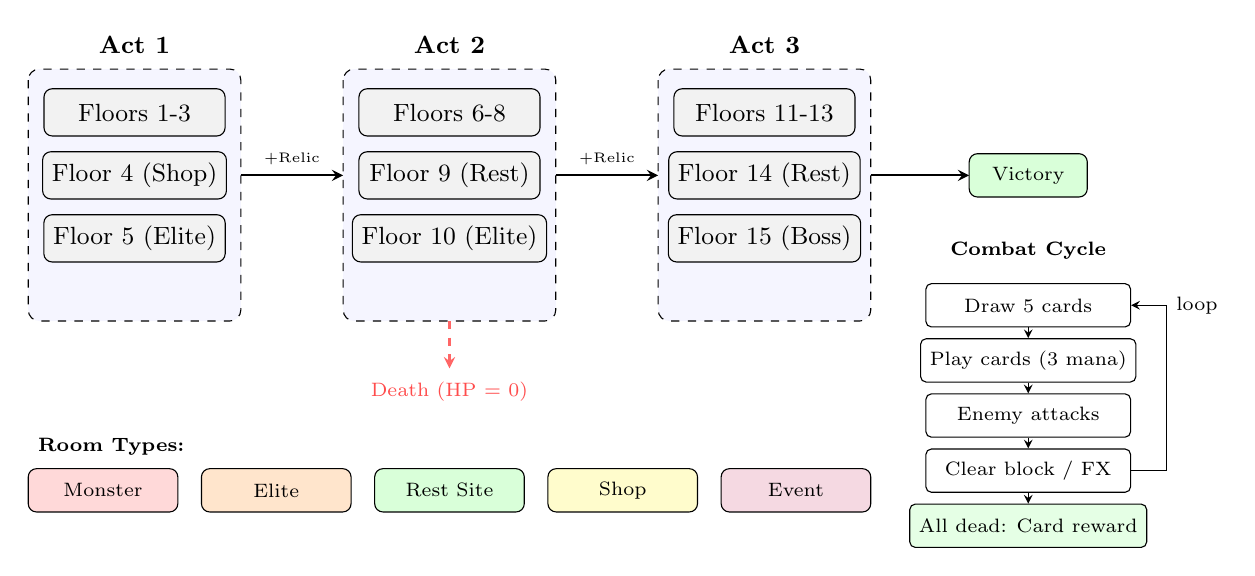
\begin{tikzpicture}[
    font=\small,
    box/.style={draw, rounded corners=3pt, minimum width=2.3cm, minimum height=0.6cm,
                text centered, fill=gray!10},
    roombox/.style={draw, rounded corners=3pt, minimum width=1.9cm, minimum height=0.55cm,
                text centered, font=\scriptsize},
    actlabel/.style={font=\small\bfseries},
    arrow/.style={->, >=stealth, thick},
    carrow/.style={->, >=stealth, thin},
    cbox/.style={draw, rounded corners=2pt, minimum width=2.6cm,
                 minimum height=0.55cm, text centered, font=\scriptsize, fill=white}
]

%--------
% LEFT PART: three-act run structure
%--------
% Act 1 bounding box
\draw[dashed, rounded corners=4pt, fill=blue!4]
    (-1.35, 2.1) rectangle (1.35, -1.1);
\node[actlabel] at (0, 2.4) {Act 1};
\node[box] at (0,  1.55) {Floors 1-3};
\node[box] at (0,  0.75) {Floor 4 (Shop)};
\node[box] at (0, -0.05) {Floor 5 (Elite)};

% Act 2 bounding box
\draw[dashed, rounded corners=4pt, fill=blue!4]
    (2.65, 2.1) rectangle (5.35, -1.1);
\node[actlabel] at (4.0, 2.4) {Act 2};
\node[box] at (4.0,  1.55) {Floors 6-8};
\node[box] at (4.0,  0.75) {Floor 9 (Rest)};
\node[box] at (4.0, -0.05) {Floor 10 (Elite)};

% Act 3 bounding box
\draw[dashed, rounded corners=4pt, fill=blue!4]
    (6.65, 2.1) rectangle (9.35, -1.1);
\node[actlabel] at (8.0, 2.4) {Act 3};
\node[box] at (8.0,  1.55) {Floors 11-13};
\node[box] at (8.0,  0.75) {Floor 14 (Rest)};
\node[box] at (8.0, -0.05) {Floor 15 (Boss)};

% Act-to-act arrows (aligned with middle row at y=0.75)
\draw[arrow] (1.35, 0.75) -- (2.65, 0.75) node[midway, above, font=\tiny] {+Relic};
\draw[arrow] (5.35, 0.75) -- (6.65, 0.75) node[midway, above, font=\tiny] {+Relic};

% Victory outcome (same row as arrows)
\draw[arrow] (9.35, 0.75) -- (10.6, 0.75);
\node[draw, rounded corners=3pt, fill=green!15, font=\scriptsize,
      minimum width=1.5cm, minimum height=0.55cm, text centered]
    at (11.35, 0.75) {Victory};

% Death outcome
\draw[arrow, dashed, draw=red!60] (4.0, -1.1) -- (4.0, -1.7);
\node[font=\scriptsize, text=red!70] at (4.0, -2.0) {Death (HP $=$ 0)};

%--------
% ROOM TYPES LEGEND (evenly spaced under all three acts)
%--------
\node[font=\scriptsize\bfseries, anchor=west] at (-1.35, -2.7) {Room Types:};
\node[roombox, fill=red!15]    at (-0.4, -3.25) {Monster};
\node[roombox, fill=orange!20] at ( 1.8, -3.25) {Elite};
\node[roombox, fill=green!15]  at ( 4.0, -3.25) {Rest Site};
\node[roombox, fill=yellow!20] at ( 6.2, -3.25) {Shop};
\node[roombox, fill=purple!15] at ( 8.4, -3.25) {Event};

%--------
% COMBAT CYCLE (right column, equal 0.70 spacing)
%--------
\node[font=\scriptsize\bfseries] at (11.35, -0.2) {Combat Cycle};
\node[cbox] (cd1) at (11.35, -0.9)  {Draw 5 cards};
\node[cbox] (cd2) at (11.35, -1.6)  {Play cards (3 mana)};
\node[cbox] (cd3) at (11.35, -2.3)  {Enemy attacks};
\node[cbox] (cd4) at (11.35, -3.0)  {Clear block / FX};
\node[cbox, fill=green!10] (cd5) at (11.35, -3.7) {All dead: Card reward};

\draw[carrow] (cd1) -- (cd2);
\draw[carrow] (cd2) -- (cd3);
\draw[carrow] (cd3) -- (cd4);
\draw[carrow] (cd4) -- (cd5);
\draw[carrow] (cd4.east) -- +(0.45,0) |- (cd1.east)
    node[pos=0.5, right, font=\scriptsize] {loop};

\end{tikzpicture}
\caption{Overview of the Roguelike Deckbuilder prototype used in this thesis. A run proceeds through three Acts (15 floors total). Each floor presents one of five room types (legend, bottom left); Monster and Elite rooms trigger the turn-based combat cycle (bottom right), which awards a new card upon victory. The run ends in Victory on defeating the Floor-15 Boss, or Death when HP reaches zero.}
\label{fig:game_overview}
\end{figure}

\section{Reinforcement Learning}

\subsection{Why RL for Sub-Problem 2: Intelligent Game Evaluation}

Sub-Problem~2 requires agents that can play the game and produce a meaningful quality signal for the optimizer. Several approaches were considered:

\textbf{Rule-based scripted agents} (the Deterministic Heuristic Agent, Section~2.4) are fast and fully deterministic, making them ideal for optimization throughput. However, a fixed rule set cannot adapt to qualitatively different game configurations: if the optimizer creates a configuration where a previously dominant card becomes weak, the DHA's rules may produce a misleading fitness estimate.

\textbf{Monte Carlo Tree Search (MCTS)} explores future states by sampling random rollout trajectories. While powerful in two-player games such as Go \cite{silver2016mastering}, MCTS is computationally prohibitive for our setting: a 15-floor run involves hundreds of sequential decisions, making per-step MCTS impractical within the optimization time budget.

\textbf{Reinforcement Learning (RL)} trains a parameterized policy directly from simulation experience, allowing the agent to learn behavioral strategies from data rather than encoding them manually. RL policies generalize to new configurations if trained with sufficient distribution coverage (addressed via Domain Randomization, Section~1.2.7). By training four RL personas with distinct reward functions, we obtain an evaluation ensemble that collectively approximates a diverse player population, surfacing balance problems that any single evaluator would miss. This ensemble is used as the validation oracle after optimization (Section~4.5).

The following subsections develop the RL theoretical framework that underlies this design: the Markov Decision Process (MDP) formalism, Deep RL, Proximal Policy Optimization (PPO), invalid action masking, and Domain Randomization.

\subsection{Markov Decision Processes}

Reinforcement Learning (RL) is the branch of machine learning concerned with training an agent to make sequential decisions in an environment by maximizing a cumulative reward signal \cite{sutton2018reinforcement}. The formal framework is the Markov Decision Process (MDP), defined as a tuple $(\mathcal{S}, \mathcal{A}, \mathcal{P}, \mathcal{R}, \gamma)$:
\begin{itemize}
    \item $\mathcal{S}$: state space - the set of all observable configurations of the environment.
    \item $\mathcal{A}$: action space - the set of possible agent actions.
    \item $\mathcal{P}(s' \mid s, a)$: transition dynamics - the probability of transitioning to state $s'$ upon taking action $a$ in state $s$.
    \item $\mathcal{R}(s, a, s')$: reward function - the immediate scalar signal received after each transition.
    \item $\gamma \in [0, 1)$: discount factor - controls the relative importance of future versus immediate rewards.
\end{itemize}

The agent's behavior is characterized by a policy $\pi(a \mid s)$, which is a probability distribution over actions conditioned on the current state. The objective is to find the optimal policy $\pi^*$ that maximizes the expected discounted return:
\begin{equation}
J(\pi) = \mathbb{E}_\pi \left[ \sum_{t=0}^{\infty} \gamma^t r_t \right]
\end{equation}

\subsection{Mapping the MDP to Our Game}

Before describing specific algorithms, it is important to ground the abstract MDP components in the concrete context of our Roguelike Deckbuilder. This mapping clarifies the design choices made in Chapter 2.

\begin{itemize}
    \item $\mathcal{S}$ - State space: At each decision point the AI agent observes a 152-dimensional vector encoding the current hero HP, block, and mana; active status effects; the cards in the current hand (up to 10 slots with 7 features each); deck composition; all enemies with their HP, block, and intended next action; equipped relics; and map context (current floor, act, available next rooms). This vector fully captures the information needed for a decision, satisfying the Markov property.
    \item $\mathcal{A}$ - Action space: The AI agent chooses from 67 discrete actions at each step: play one of up to 10 hand cards (with or without a specific enemy target), end the player turn, navigate to one of the available next-room nodes, use a health potion, or select a card reward. An action mask vector of length 67 marks illegal actions at each step (e.g., playing a card when mana is insufficient).
    \item $\mathcal{P}(s' \mid s, a)$ - Transition dynamics: The game engine is deterministic given a fixed random seed, but stochastic in practice because card draws, enemy intent patterns, and reward pools are randomized each run. This stochasticity requires the AI agent to plan for uncertainty rather than memorize a fixed sequence of actions.
    \item $\mathcal{R}(s, a, s')$ - Reward function: Four distinct reward functions are used, one per agent persona. Each shapes behavior toward a specific play style (Aggressive, Defensive, Balanced, Adaptive) through different weightings of events such as enemy kills, HP loss, block gained, and floor progression. The detailed reward functions are defined in Section~\ref{sec:agent_design}.
    \item $\gamma$ - Discount factor: We use $\gamma = 0.99$. A 15-floor run involves hundreds of decision steps, so a high discount factor is necessary for the AI agent to reason about late-game consequences. A low value such as $\gamma = 0.9$ would cause the agent to ignore floor-10 to floor-15 outcomes almost entirely.
\end{itemize}

\subsection{Deep Reinforcement Learning}

In environments with large or continuous state spaces (such as our game, with a 152-dimensional observation vector), the policy is parameterized by a deep neural network $\pi_\theta(a \mid s)$. The action-value function $Q^\pi(s, a)$ and state-value function $V^\pi(s)$ are defined as:
\begin{align}
Q^\pi(s, a) &= \mathbb{E}_\pi \left[ \sum_{t=0}^{\infty} \gamma^t r_t \,\Big|\, s_0=s, a_0=a \right] \\
V^\pi(s) &= \mathbb{E}_{a \sim \pi} \left[ Q^\pi(s, a) \right]
\end{align}
The advantage function $A^\pi(s, a) = Q^\pi(s, a) - V^\pi(s)$ measures how much better action $a$ is compared to the average under policy $\pi$.

\subsection{Proximal Policy Optimization (PPO)}

PPO \cite{schulman2017proximal} is an on-policy actor-critic algorithm that achieves stable policy updates by constraining the ratio between the updated and old policy:
\begin{equation}
\mathcal{L}^{\text{CLIP}}(\theta) = \mathbb{E}_t \left[ \min\!\left( r_t(\theta) \hat{A}_t,\; \text{clip}(r_t(\theta), 1-\epsilon, 1+\epsilon)\, \hat{A}_t \right) \right]
\label{eq:ppo_clip}
\end{equation}
where $r_t(\theta) = \frac{\pi_\theta(a_t \mid s_t)}{\pi_{\theta_\text{old}}(a_t \mid s_t)}$ is the probability ratio, $\hat{A}_t$ is the estimated advantage, and $\epsilon$ (typically 0.1 - 0.2) is the clipping range. PPO is widely adopted in practice due to its simplicity, sample efficiency relative to trust-region methods, and ease of parallelization \cite{schulman2017proximal}.

The full PPO objective combines the clipped policy loss with a value function regression loss and an entropy bonus:
\begin{equation}
\mathcal{L}^{\text{PPO}}(\theta) = \mathbb{E}_t \left[ \mathcal{L}^{\text{CLIP}}(\theta) - c_1 \mathcal{L}^{\text{VF}}(\theta) + c_2 H[\pi_\theta](s_t) \right]
\label{eq:ppo_full}
\end{equation}
where $c_1$ and $c_2$ are coefficients for value loss and entropy bonus, respectively. The entropy term $H[\pi_\theta]$ encourages exploration by penalizing overly deterministic policies.

\subsection{Invalid Action Masking}

In environments with discrete action spaces subject to game-rule constraints, many actions may be illegal at any given step (e.g., playing a card when insufficient mana is available). Training vanilla PPO in such environments wastes sample efficiency as the agent must learn the constraints from scratch.

Invalid Action Masking \cite{huang2020closer} eliminates illegal actions before policy probability computation by setting the logits of masked actions to $-\infty$ before the softmax:
\begin{equation}
\pi_\theta(a \mid s) = \text{softmax}\!\left( \mathbf{z} + \mathbf{m} \right),\quad m_i = \begin{cases} 0 & \text{if action } i \text{ is valid} \\ -\infty & \text{otherwise} \end{cases}
\end{equation}
This approach is theoretically equivalent to valid policy gradient updates \cite{huang2020closer} and dramatically accelerates learning in constraint-heavy environments such as deckbuilding games. The \textit{sb3-contrib} library provides \textit{MaskablePPO}, a drop-in extension of Stable-Baselines3~\cite{raffin2021stable} PPO that natively supports action masking.

\subsection{Domain Randomization}

Domain Randomization (DR) was originally proposed to transfer robot policies trained in simulation to the physical world \cite{tobin2017domain}. The key insight is that if a policy is trained across a distribution of simulation environments (parameterized by varying physics, lighting, or object properties), it may generalize to the real world as merely another sample from that distribution.

In our context, DR serves a different but analogous purpose: because the NSGA-II optimization modifies game parameters across a bounded range, the RL agents must remain competent across all configurations in that range, not just the nominal one. At each environment \textit{reset()}, we add uniform noise $\epsilon \sim \mathcal{U}(-\delta, \delta)$ to each game parameter:
\begin{equation}
\tilde{\theta}_i = \theta_i \cdot (1 + \epsilon_i), \quad \epsilon_i \sim \mathcal{U}(-\delta, \delta)
\end{equation}
This forces agents to learn behavioral policies based on relative relationships (e.g., ``play the highest-damage card relative to enemy HP'') rather than memorizing absolute parameter values, making them robust evaluators for any point in the optimization search space.

\section{Optimization Algorithms}

This section addresses Sub-Problem~3: automated search over the game parameter space for configurations that simultaneously satisfy the Balance, Engagement, and Coherence objectives. We first survey the landscape of automated game balancing approaches to motivate the choice of evolutionary methods, then present the single-objective Genetic Algorithm (Section~1.3.2) and the multi-objective NSGA-II (Section~1.3.3).

\subsection{Survey of Automated Game Balancing Approaches}

Before introducing the specific algorithms used in this thesis, it is useful to survey the landscape of automated game balancing approaches. This positions the choice of evolutionary algorithms and makes explicit why simpler alternatives are insufficient for Sub-Problem~3.

\textbf{Manual playtesting} is the baseline industry approach: designers adjust parameters by hand based on player feedback. While it captures nuanced human perception, it does not scale - a 500-parameter space requires exponentially many sessions to explore systematically, and each iteration takes days or weeks of design time.

\textbf{Hill-climbing and local search} start from an initial configuration and iteratively perturb one parameter at a time, accepting changes that improve a scalar fitness score. These methods are easy to implement but are highly susceptible to local optima in non-convex, high-dimensional landscapes, and they cannot handle competing objectives without collapsing them into a single weighted sum.

\textbf{Simulated annealing} extends hill-climbing with a temperature schedule that occasionally accepts worse solutions, enabling escape from local optima. However, it still requires a single scalar fitness function, losing the trade-off information between Balance, Engagement, and Coherence that a Pareto front preserves.

\textbf{Coevolutionary methods} evolve both game parameters and agent strategies simultaneously, using inter-agent competition dynamics as a balance signal \cite{nelson2007towards}. While theoretically elegant, coevolution is notoriously unstable: the fitness landscape shifts as agents co-adapt, making convergence unreliable without carefully tuned population sizes and update schedules.

\textbf{Evolutionary Algorithms (EA)} address the key shortcomings above. By maintaining a \emph{population} of candidate solutions, EAs explore the search space globally rather than locally; crossover recombines partial solutions from fit individuals to discover configurations that neither parent achieves alone; elitism preserves the best solutions found. For our 500-dimensional continuous parameter space with three competing objectives, EAs are the most suitable class of methods. Section~1.3.2 presents the single-objective GA; Section~1.3.3 extends this to the multi-objective NSGA-II, which returns a Pareto front rather than a single solution.

\subsection{Genetic Algorithms}

Genetic Algorithms (GA) are a family of population-based metaheuristics that abstract the mechanisms of biological evolution \cite{holland1992adaptation}. A GA maintains a population of candidate solutions (genomes), evaluates their fitness with respect to an objective function, and iteratively applies selection, crossover, and mutation operators to produce progressively better populations. The key insight is that combining partial solutions from fit individuals (crossover) can discover configurations that neither parent achieves alone, while random perturbations (mutation) prevent premature convergence to local optima.

\subsubsection{Core Components}

Genome representation encodes a candidate solution as a chromosome. For continuous optimization problems, genomes are vectors of real numbers $\mathbf{g} = (g_1, g_2, \ldots, g_n) \in \mathbb{R}^n$. In our game-balancing application, each gene $g_i$ is a multiplier applied to a specific game parameter (e.g., the base damage of a particular card).

Fitness function $f: \mathbb{R}^n \to \mathbb{R}$ assigns a scalar quality score to each genome. For single-objective GA:
\begin{equation}
F(\mathbf{g}) = w_1 \cdot f_{\text{balance}}(\mathbf{g}) + w_2 \cdot f_{\text{engagement}}(\mathbf{g}) + w_3 \cdot f_{\text{coherence}}(\mathbf{g})
\label{eq:ga_fitness}
\end{equation}
\begin{sloppypar}
where $w_1, w_2, w_3$ are pre-determined weights. In our game-balancing application (Sub-Problem~3), each term maps directly to a simulation-derived quantity:
\end{sloppypar}
\begin{itemize}
    \item $f_{\text{balance}}(\mathbf{g})$: a score in $[0,1]$ measuring how closely the AI agent win rate, average victory HP, and average floor-on-death align with designer-specified targets (45\%, 30\%, and Floor~10, respectively). It is computed by the \textit{FitnessEvaluator} from batch simulation statistics.
    \item $f_{\text{engagement}}(\mathbf{g})$: a score in $[0,1]$ measuring the fraction of cards that are genuinely viable - i.e., picking them correlates positively with winning. A configuration where only 3 out of 30 cards are worth picking scores near 0; one where all 30 are competitive scores near 1.
    \item $f_{\text{coherence}}(\mathbf{g})$: a score in $[0,1]$ penalizing trap cards (high pick rate but below-average win contribution) and parameter values outside an interpretable range. A configuration with no trap cards and all scaling multipliers in $[0.5,\,2.0]$ scores near 1.
    \item $w_1=0.5,\;w_2=0.3,\;w_3=0.2$: designer-chosen weights reflecting that balance is the primary concern, followed by engagement and coherence. These weights are fixed before optimization, which is a key limitation of the single-objective GA addressed by NSGA-II in Section~1.3.3.
\end{itemize}

Selection determines which genomes reproduce. Tournament selection of size $k$ draws $k$ individuals uniformly at random and returns the fittest, providing tunable selection pressure without requiring global fitness ranking.

Crossover combines two parent genomes to produce offspring. Uniform crossover assigns each gene to offspring 1 or offspring 2 with probability 0.5, effectively sampling a random hypercube between the two parents:
\begin{equation}
g_i^{\text{child}} = \begin{cases} g_i^{P_1} & \text{with probability } 0.5 \\ g_i^{P_2} & \text{with probability } 0.5 \end{cases}
\end{equation}

Mutation perturbs genes stochastically to maintain diversity. Gaussian mutation adds zero-mean noise:
\begin{equation}
g_i' = g_i + \mathcal{N}(0, \sigma^2), \quad \text{with probability } p_m
\label{eq:gaussian_mutation}
\end{equation}
Typical values are $p_m \in [0.01, 0.05]$ and $\sigma \in [0.05, 0.2]$ for normalized parameter ranges.

Elitism preserves a fraction of the top individuals unchanged across generations, ensuring that the best discovered solution never degrades.

\subsection{NSGA-II: Multi-Objective Evolutionary Optimization}

While the GA (Section~1.3.2) uses a fixed weighted sum of objectives, this collapses the multi-dimensional trade-off space into a single number determined by the designer's prior weighting. NSGA-II addresses this limitation by returning a full Pareto front of non-dominated solutions in a single run, giving the designer a post-hoc menu of configurations to choose from.

\subsubsection{Why Multi-Objective Optimization for Game Balancing?}

Several paradigms exist for optimizing problems with multiple competing objectives. \textbf{Weighted-sum scalarization} (used by the single-objective GA, Section~1.3.2) converts all objectives into a single scalar; it is computationally cheap but requires committing to fixed weights $w_i$ before optimization, which pre-determines the trade-off without seeing the actual design space. \textbf{$\varepsilon$-constraint methods} optimize one objective while bounding the others as inequality constraints; each run produces a single Pareto-optimal point, requiring $k$ runs to trace $k$ points on the front. \textbf{Decomposition-based methods} (e.g., MOEA/D) decompose the problem into scalar subproblems along a grid of weight vectors; they are efficient but still require the designer to pre-specify the weight grid. \textbf{Pareto-based evolutionary methods} - of which NSGA-II is the canonical example - maintain a population of non-dominated solutions and return the full Pareto front in a single run; they are the natural choice when the designer's preference ordering is unknown a priori.

\begin{sloppypar}
For our game-balancing problem, a Pareto-based approach is preferred for two reasons. First, no weight vector can fully capture designer intent across all possible game audiences: a configuration targeting casual players prioritizes engagement over strict balance, while a competitive-mode configuration inverts these priorities. Second, revealing the actual trade-off curve allows the designer to make an informed post-hoc selection - a qualitatively richer outcome than a single number.
\end{sloppypar}

A straightforward alternative to NSGA-II is a weighted-sum fitness function: $F = w_1 \cdot \text{Balance} + w_2 \cdot \text{Engagement} + w_3 \cdot \text{Coherence}$. This is exactly what the single-objective GA in this thesis implements with weights $(0.5, 0.3, 0.2)$. The limitation is that the weights must be chosen before optimization runs, but no single weight vector is universally correct: a game designer targeting tournament play might prioritize balance above all, while one targeting casual players might prefer high engagement even at a small cost to balance.

NSGA-II avoids this limitation by treating all three objectives as separate criteria and returning a \textit{Pareto front} - a set of solutions where improving one objective necessarily degrades at least one other. The designer inspects this front \textit{after} seeing the actual trade-off space and selects the solution matching their priorities. This post-hoc selection is far more informative than blindly pre-specifying weights.

A second advantage is search diversity: NSGA-II's crowding distance mechanism actively maintains a spread of solutions across the Pareto front, preventing the population from collapsing onto a single region of the objective space. In game balancing, where the interaction between Balance, Engagement, and Coherence is non-linear and hard to predict, this diversity is essential for discovering unexpected high-quality configurations.

\subsubsection{Multi-Objective Problem Formulation}

Many real-world optimization problems require simultaneously maximizing several objectives that are in mutual tension \cite{deb2002fast,coello2007evolutionary}. The general multi-objective optimization problem is:
\begin{equation}
\text{maximize} \quad \mathbf{F}(\mathbf{x}) = \bigl(f_1(\mathbf{x}),\, f_2(\mathbf{x}),\, \ldots,\, f_m(\mathbf{x})\bigr)
\end{equation}
Because improving one objective typically harms another, there is no single ``optimal'' solution. Instead, the goal is to characterize the Pareto front - the set of solutions that are non-dominated.

\begin{definition}[Pareto Dominance]
Solution $\mathbf{x}_1$ dominates $\mathbf{x}_2$ (written $\mathbf{x}_1 \prec \mathbf{x}_2$) if and only if:
\begin{equation}
\forall i : f_i(\mathbf{x}_1) \geq f_i(\mathbf{x}_2) \quad \text{and} \quad \exists j : f_j(\mathbf{x}_1) > f_j(\mathbf{x}_2)
\end{equation}
\end{definition}

\begin{definition}[Pareto Optimal Set]
A solution $\mathbf{x}^*$ is Pareto optimal if no solution in the feasible space dominates it. The set of all Pareto optimal solutions forms the Pareto front.
\end{definition}

\subsubsection{The NSGA-II Algorithm}

NSGA-II (Non-dominated Sorting Genetic Algorithm II), proposed by Deb et al.\ \cite{deb2002fast}, is the canonical multi-objective evolutionary algorithm. Its three key innovations over the original NSGA are: (1) efficient $\mathcal{O}(MN^2)$ fast non-dominated sorting, where $M$ is the number of objectives and $N$ is the population size; (2) a crowding distance metric for diversity preservation; and (3) an elitist selection strategy.

Fast non-dominated sorting partitions the population $P$ into fronts $\mathcal{F}_1, \mathcal{F}_2, \ldots$ where $\mathcal{F}_1$ contains all non-dominated individuals, $\mathcal{F}_2$ those dominated only by members of $\mathcal{F}_1$, and so on. The rank of individual $i$ equals its front index.

Crowding distance $d_i$ measures the density of solutions surrounding individual $i$ in objective space:
\begin{equation}
d_i = \sum_{k=1}^{m} \frac{f_k^{(i+1)} - f_k^{(i-1)}}{f_k^{\max} - f_k^{\min}}
\label{eq:crowding_distance}
\end{equation}
where $i \pm 1$ denotes the adjacent individuals when sorted by objective $k$. Boundary solutions receive $d_i = \infty$.

NSGA-II selection operator $\prec_n$ prefers lower rank, breaking ties by larger crowding distance:
\begin{equation}
\mathbf{x}_1 \prec_n \mathbf{x}_2 \iff \text{rank}(\mathbf{x}_1) < \text{rank}(\mathbf{x}_2) \;\text{ or }\; \bigl(\text{rank}(\mathbf{x}_1) = \text{rank}(\mathbf{x}_2) \text{ and } d_1 > d_2\bigr)
\end{equation}
This guarantees convergence toward the Pareto front while maintaining diversity along it.

Simulated Binary Crossover (SBX) and Polynomial Mutation are the preferred genetic operators for real-valued chromosomes in NSGA-II. SBX mimics single-point crossover for binary representations but operates directly on floating-point variables \cite{deb2002fast}.

\section{Related Work}

\subsection{Automated Game Balancing}

Nelson and Mateas \cite{nelson2007towards} proposed a broader framework for automated game design, though primarily for simple rule-based games.

Our work distinguishes itself from this body of literature by (1) addressing the more complex Deckbuilder sub-genre, (2) employing four learned RL personas instead of scripted evaluation bots, and (3) providing a systematic empirical comparison between a flat single-objective GA and a structured multi-objective NSGA-II under identical simulation budgets.

\subsection{RL for Card Games}

Reinforcement learning has been successfully applied to complex card games. AlphaStar demonstrated superhuman performance in StarCraft II using a combination of imitation learning and self-play \cite{vinyals2019grandmaster}. The foundational DQN algorithm \cite{mnih2015human} has since been applied to discrete card-game environments such as Dominion, while PPO-family algorithms have been explored in simplified Slay the Spire variants. Both lines of work confirm that deep RL is well suited to the discrete, constraint-heavy action spaces of card games, but neither connected agent training to systematic game balancing - a gap this thesis directly addresses.

\subsection{Procedural Content Generation}

Togelius et al.\ \cite{togelius2011search} provide a comprehensive survey of search-based PCG, demonstrating that evolutionary approaches are effective at generating game content that satisfies multiple quality criteria. Preuss et al.\ \cite{preuss2012multiobjective} apply multi-objective optimization specifically to PCG, a setting directly analogous to our balancing problem. Our contribution complements this line of work by focusing on parameter tuning (rather than content generation) and by using RL agents as the evaluation oracle.
